%!TEX root = ../thesis.tex
%*******************************************************************************
%*********************************** Third Chapter *****************************
%*******************************************************************************

\chapter{Biological aspects of the epigenetic clock}  \label{c:3}

\ifpdf
    \graphicspath{{Chapter3/Figs/Raster/}{Chapter3/Figs/PDF/}{Chapter3/Figs/}}
\else
    \graphicspath{{Chapter3/Figs/Vector/}{Chapter3/Figs/}}
\fi


%********************************** %First Section  **************************************
\section{Background} 

\smallskip

Epigenetic clocks can be understood as a proxy to quantify the changes of the epigenome with age. However, little is known about the molecular mechanisms that determine the rate of these clocks. Steve Horvath proposed that the multi-tissue epigenetic clock captures the workings of an \textbf{epigenetic maintenance system} \cite{Horvath2013}. Recent \acrshort{GWAS} studies have found several genetic variants associated with epigenetic age acceleration in genes such as \textit{TERT} (the catalytic subunit of telomerase) \cite{Lu2018}, \textit{DHX57} (an ATP-dependent RNA helicase) \cite{Lu2016} or \textit{MLST8} (a subunit of both mTORC1 and mTORC2 complexes) \cite{Lu2016}. Nevertheless, to my knowledge no genetic variants in epigenetic modifiers have been found and the molecular nature of this hypothetical system is unknown to this date.

\bigskip

I decided to take a reverse genetics approach and look at the \textbf{behaviour of the epigenetic clock in patients with developmental disorders}, many of which harbour mutations in proteins of the epigenetic machinery \cite{Aref-Eshghi2018,Bjornsson2015}. I performed an unbiased screen for epigenetic age acceleration and found that Sotos syndrome accelerates epigenetic ageing, potentially revealing a role of H3K36 methylation maintenance in the regulation of the rate of the epigenetic clock.

\smallskip

\section{Screening for genes that accelerate the epigenetic clock} \label{s:3.2}

\smallskip

The main goal of this analysis is to identify genes, mainly components of the epigenetic machinery, that can \textbf{affect the rate of epigenetic ageing in humans} (as measured by Horvath’s epigenetic clock) \cite{Horvath2013}. For this purpose, I assembled a dataset with all the DNA methylation data from patients with different developmental disorders that I could find, in order to perform an unbiased screen. This dataset combines samples publicly available in GEO \cite{Edgar2002} with in-house data generated by my collaborators in the London Health Sciences Centre, Canada (Table~\ref{table:s2_table1}, Fig.~\ref{fig:sc3_fig1}). All the data were generated from blood using the 450K methylation array, as in the case of the healthy individuals described in Chapter~\ref{c:2}.   

\bigskip

Many of these developmental syndromes present overlap of some of their clinical features \cite{Aref-Eshghi2018, Bjornsson2015}. Furthermore, in some cases with a clinical diagnosis, the genetic cause remains unknown, probably due to locus heterogeneity or difficulty to assess the clinical significance of some genetic variants \cite{Aref-Eshghi2017}. Therefore, several studies have explored the ability of DNA methylation signatures to aid differential diagnoses of these syndromes \cite{Aref-Eshghi2018,Aref-Eshghi2017,Aref-Eshghi2018a,Butcher2017,Choufani2015,Schenkel2016,Alisch2013,Schenkel2017,Hood2016,Aldinger2013,Grafodatskaya2013,Kernohan2016}. Given that most of the diagnoses for developmental disorders are carried out early in life, this led to a dataset with a bias towards younger ages (Fig.~\ref{fig:c3_fig1}). In order to maximise the ability to detect ageing-associated effects, I kept only those developmental disorders that had at least 5 samples, with 2 of them with an age $\geq 20$ years (which, according to Horvath's model, is the adult age for humans) \cite{Horvath2013}. This filtering resulted in a dataset for the main screen with $N = 367$ samples from cases, which had ages between 0 and 55 years (Fig.~\ref{fig:c3_fig2}, Table~\ref{table:c3_table1}).

\begin{figure}[htbp!] 
	\centering
	\vspace*{6mm}    
	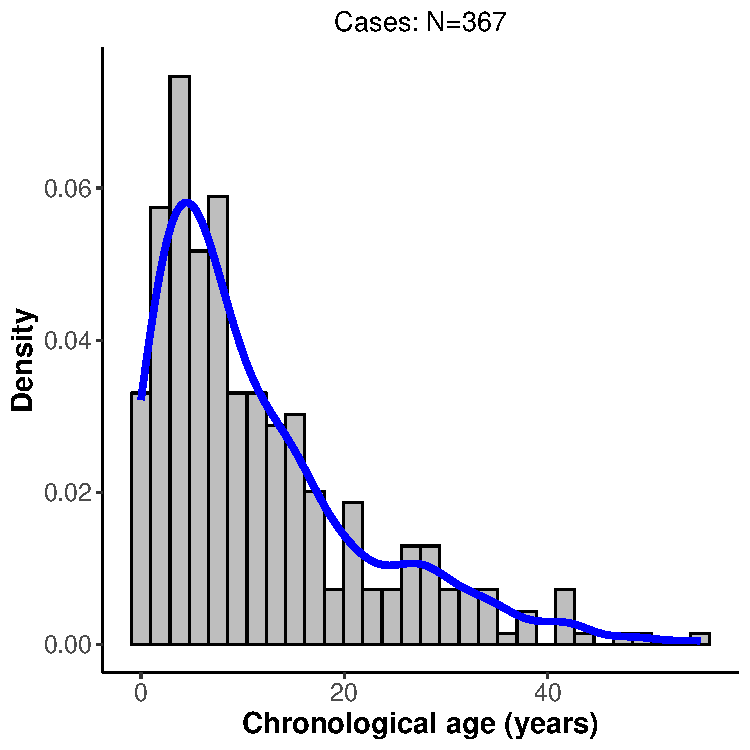
\includegraphics[width=0.6\textwidth]{C3_Fig1}
	\vspace*{2mm}
	\caption[Chronological age distribution in the individuals with developmental disorders]{Histogram showing the chronological age distribution for all the individuals with developmental disorders (cases) included in the final dataset (i.e. after QC and filtering). The blue line represents the 1D kernel density estimate, as calculate by the \textit{stat\_density} function in R with default parameters.}
	\label{fig:c3_fig1}
\end{figure}

\begin{figure}[htbp!] 
	\centering    
	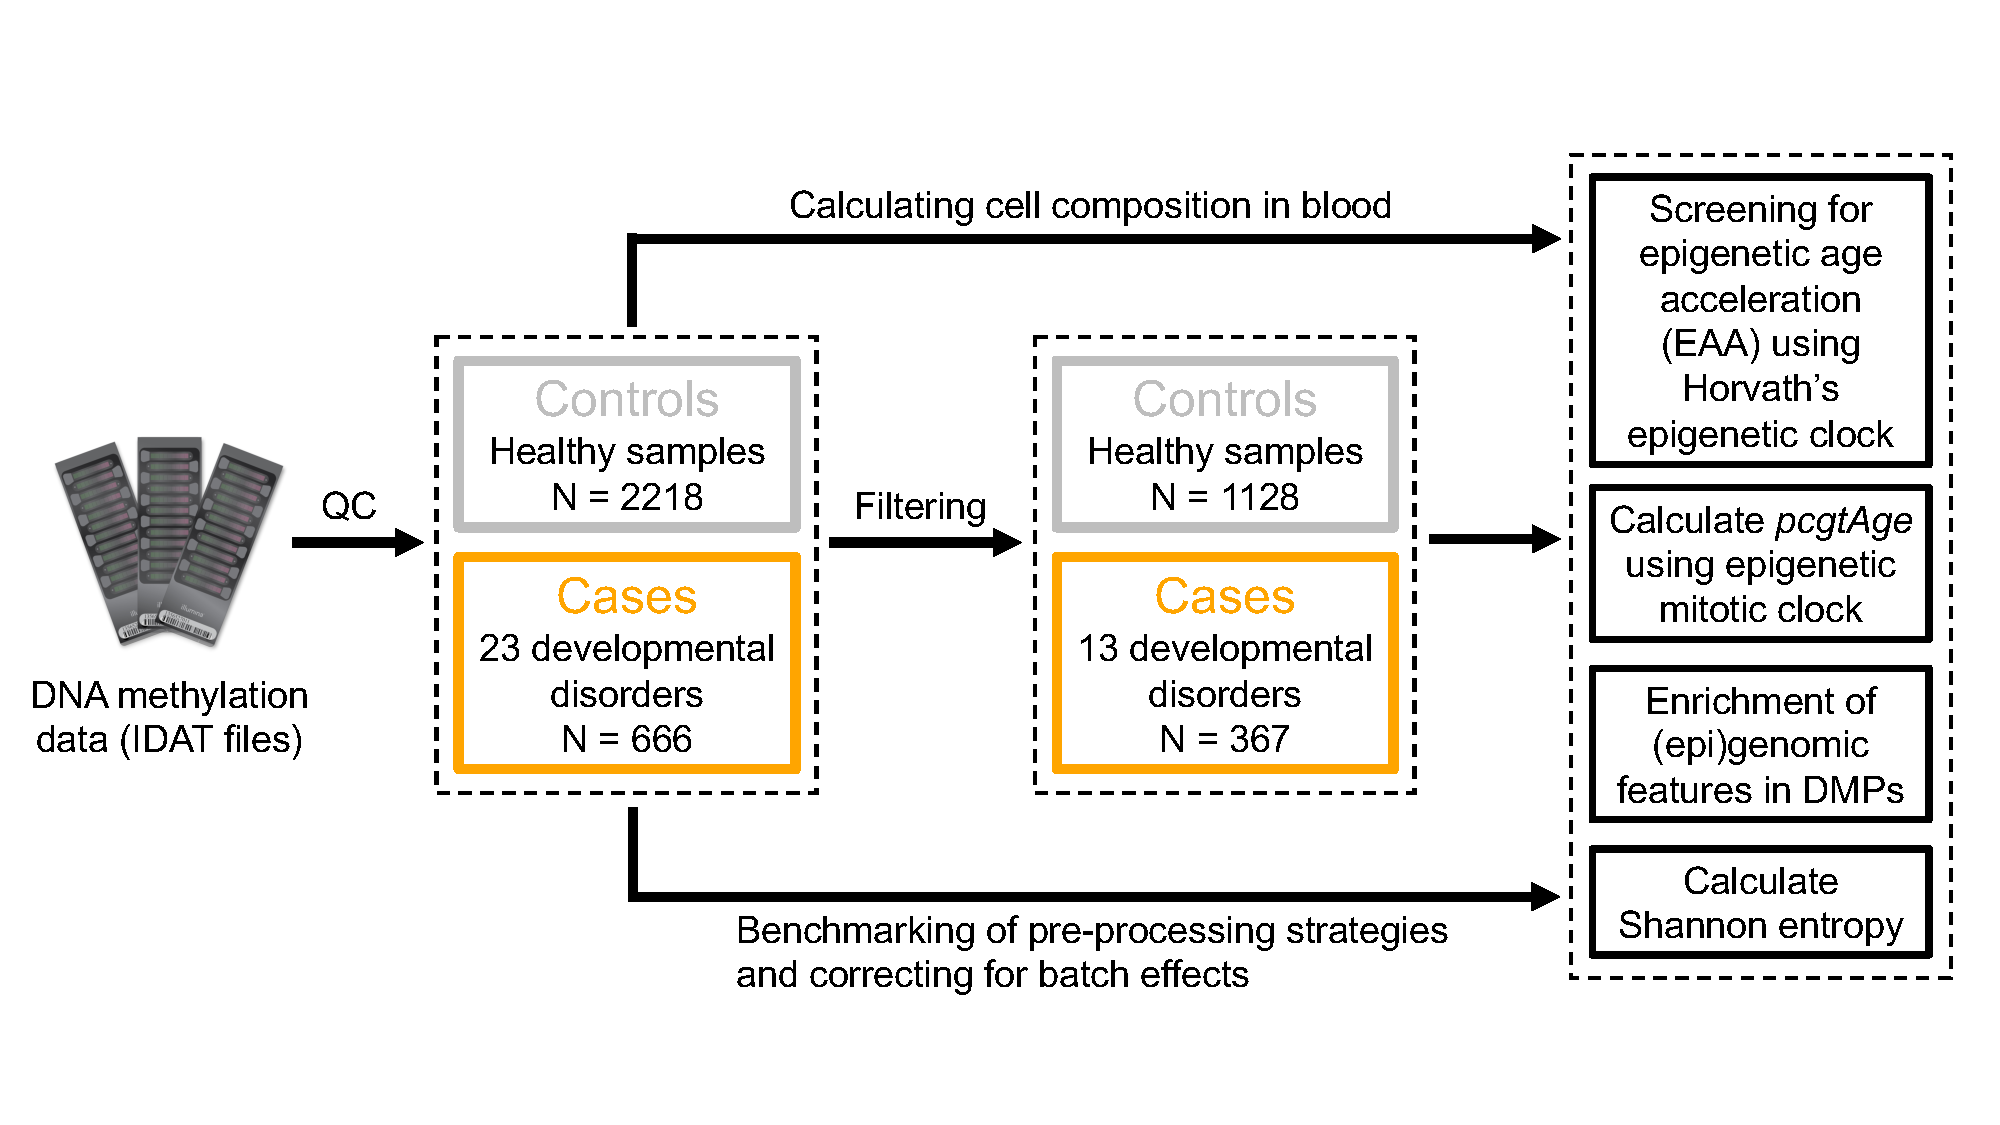
\includegraphics[width=1\textwidth]{C3_Fig2}
	\caption[Overview of the analyses performed in Chapter~\ref{c:3}]{Flow diagram that portrays an overview of the different analyses that are carried out in the raw DNA methylation data (IDAT files) from human blood for cases (developmental disorders samples) and controls (healthy samples). The control samples are filtered to match the age range of the cases (0-55 years). The cases are filtered based on the number of `adult’ samples available (for each disorder, at least 5 samples, with 2 of them with an age $\geq$ 20 years). QC: quality control. DMPs: differentially methylated positions.}
	\label{fig:c3_fig2}
\end{figure}

\begin{table}
	%\centering
	\small
	\begin{tabular}{ p{4cm} p{2cm} p{2cm} p{2cm} p{1cm} p{2cm} }
		\toprule
		\textbf{Developmental disorder} & \textbf{Gene(s) involved} & \textbf{Gene(s) function} & \textbf{Molecular cause} & \textbf{N} & \textbf{Age range (years)} \\
		\midrule
		Angelman & \textit{UBE3A} & Ubiquitin protein ligase E3A & Imprinting, mutation & 14 & 1 to 55 \\
		\midrule
		Autism spectrum disorder (ASD) & - & - & - & 119 & 1.83 to 35.16 \\
		\midrule
		Alpha thalassemia/mental retardation X-linked syndrome (ATR-X) & \textit{ATRX} &Chromatin remodelling & Mutation & 15 & 0.7 to 27 \\
		\midrule
		Claes-Jensen & \textit{KDM5C} & H3K4 demethylase & Mutation & 10 & 2 to 42 \\
		\midrule
		Coffin-Lowry & \textit{RPS6KA3} & Serine / threonine kinase & Mutation & 10 & 1.3 to 22.8 \\
		\midrule
		Floating-Harbour & \textit{SRCAP} & Chromatin remodelling & Mutation & 17 & 4 to 42 \\
		\midrule
		Fragile X syndrome (FXS) & \textit{FMR1} & Translational control & Mutation (CGG expansion) & 32 & 0.08 to 48 \\
		\midrule
		Kabuki & \textit{KMT2D} & H3K4 methyltransferase & Mutation & 46 & 0 to 24.1 \\
		\midrule
		Noonan & \textit{PTPN11}, \textit{RAF1}, \textit{SOS1} & RAS/ MAPK signalling & Mutation & 15, 11, 14 & 0.2 to 49 \\
		\midrule
		Rett & \textit{MECP2} & Transcriptional repression & Mutation & 15 & 1 to 34 \\
		\midrule
		Saethre-Chotzen & \textit{TWIST1} & Transcription factor & Mutation & 22 & 0 to 38 \\
		\midrule
		Sotos & \textit{NSD1} & H3K36 methyltransferase & Mutation & 20 & 1.6 to 41 \\
		\midrule
		Weaver & \textit{EZH2} & H3K27 methyltransferase & Mutation & 7 & 2.58 to 43 \\
		\midrule
		\textbf{Total} & - & - & - & 367 & 0 to 55  \\ 
		\bottomrule
	\end{tabular}
	\vspace*{3mm}
	\caption[Overview of the developmental disorders that were included in the screening]{Overview of the developmental disorders that were included in the screening after quality control and filtering (total $N=367$).}
	\label{table:c3_table1}
\end{table} 

\bigskip

The purpose of the screen is to \textbf{test whether the epigenetic ages of the samples from a given developmental disorder (cases) deviate from their chronological age} i.e. identify those developmental disorders that present epigenetic age acceleration (EAA). For a given sample, a positive EAA indicates that the epigenetic (biological) age of the sample is higher than the one expected for someone with that chronological age. In other words, it means that the epigenome of that person resembles the epigenome of an older individual. The opposite is true when a negative EAA is found (i.e. the epigenome looks younger than expected). I calculated the epigenetic ages ($DNAmAge$) of all the samples according to Horvath's epigenetic clock (see section~\ref{s:2.2.1}) and I fitted the control models to the samples from the healthy individuals, including models with and without cell composition correction (CCC) and always accounting for potential batch effects (see equations \ref{eq:2.16} and \ref{eq:2.17}).  As previously discussed (see section~\ref{s:2.2.2}), due to the fact that Horvath's model underestimates the epigenetic age of old samples, the age distribution of the control samples can have an impact on the results of the screen. Therefore, I filtered the ages of the healthy individual samples to make them match the age range of the developmental disorders (0-55 years, $N = 1128$, see Fig.~\ref{fig:c3_fig2}).

\bigskip

The EAA for the control samples corresponds to the residuals from the control models (see section~\ref{s:2.2.2}). On the other hand, the EAA for a case sample is calculated by taking the difference between the epigenetic age ($DNAmAge$) and the predicted value from the corresponding control model (with or without cell composition). Finally, I compared the distributions of the EAA for the different developmental disorders against the EAA distributions for the healthy controls using the non-parametric two-sided Wilcoxon's test. P-values were adjusted for multiple testing using Bonferroni correction and a significance level of $\alpha = 0.01$ was applied. It is worth mentioning that some of the developmental disorders included in the screen (such as autism spectrum disorder or Coffin-Lowry syndrome) are not necessarily caused by alterations in the epigenetic machinery, but were still included to maintain the unbiased nature of the screen. 

\smallskip

\section{Sotos syndrome accelerates epigenetic ageing}

\smallskip

The results from the screen are portrayed in Fig.~\ref{fig:c3_fig3}. Most syndromes do not show evidence of accelerated epigenetic ageing, but \textbf{Sotos syndrome presents a clear positive EAA} (median EAA$_{\text{with CCC}}$ = + 7.64 years, median EAA$_{\text{without CCC}}$ = + 7.16 years), with p-values considerably below the significance level of 0.01 after Bonferroni correction (p-value$_{\text{corrected, with CCC}}$ = 3.40 $\cdot$ 10$^{-9}$, p-value$_{\text{corrected, without CCC}}$ = 2.61 $\cdot$ 10$^{-7}$). Additionally, Rett syndrome (median EAA$_{\text{with CCC}}$ = + 2.68 years, median EAA$_{\text{without CCC}}$ = + 2.46 years, p-value$_{\text{corrected, with CCC}}$ = 0.0069, p-value$_{\text{corrected, without CCC}}$ = 0.0251) and Kabuki syndrome (median EAA$_{\text{with CCC}}$ = - 1.78 years, median EAA$_{\text{without CCC}}$ = - 2.25 years, p-value$_{\text{corrected, with CCC}}$ = 0.0011, p-value$_{\text{corrected, without CCC}}$ = 0.0035) reach significance, with a positive and negative EAA respectively. Finally, fragile X syndrome (FXS) shows a positive EAA trend (median EAA$_{\text{with CCC}}$ = + 2.44 years, median EAA$_{\text{without CCC}}$ = + 2.88 years) that does not reach significance in the screen (p-value$_{\text{corrected, with CCC}}$ = 0.0680, p-value$_{\text{corrected, without CCC}}$ = 0.0693).

\bigskip

\begin{figure}[htbp!] 
	\centering    
	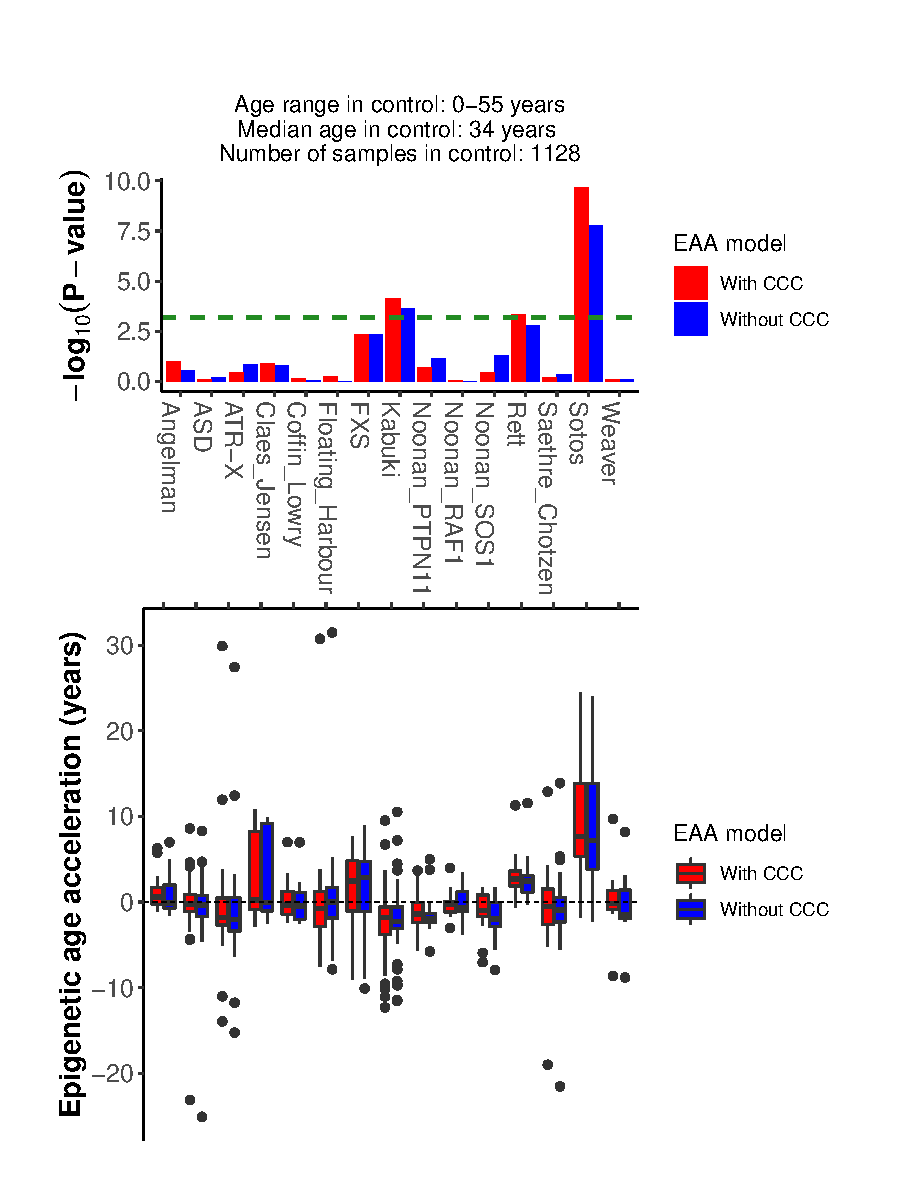
\includegraphics[width=1\textwidth]{C3_Fig3}
	\caption[Screening for epigenetic age acceleration (EAA) in developmental disorders]{Screening for epigenetic age acceleration (EAA) in developmental disorders. The upper panel shows the p-values derived from comparing the EAA distributions for the samples in a given developmental disorder and the control (two-sided Wilcoxon’s test). The dashed green line displays the significance level of $\alpha = 0.01$ after Bonferroni correction. The bars above the green line reach statistical significance. The lower panel displays the actual EAA distributions, which allows assessing the direction of the EAA (positive or negative). In red: EAA model with cell composition correction (CCC). In blue: EAA model without CCC. ASD: autism spectrum disorder. ATR-X: alpha thalassemia/mental retardation X-linked syndrome. FXS: fragile X syndrome.}
	\label{fig:c3_fig3}
\end{figure}

Next, I tested the effect of changing the median age used to build the healthy control model (i.e. the median age of the controls) on the screening results (Fig.~\ref{fig:sc3_fig2}). Sotos syndrome is robust to these changes, whilst Rett, Kabuki and FXS are much more sensitive to the control model used. This again highlights the importance of choosing an appropriate age-matched control when testing for epigenetic age acceleration, given that Horvath’s epigenetic clock underestimates epigenetic age for advanced chronological ages \cite{ElKhoury2018,Marioni2018}.

\bigskip

Moreover, all but one of the Sotos syndrome patients (19/20 = 95\%) show a consistent deviation in EAA (with CCC) in the same direction (Fig.~\ref{fig:c3_fig4}a,b), which is not the case for the rest of the disorders, with the exception of Rett syndrome (Fig.~\ref{fig:sc3_fig3}). Even though the data suggest that there are already some methylomic changes at birth, the EAA seems to increase with age in the case of Sotos patients (Fig.~\ref{fig:c3_fig4}b). This implies that at least some of the changes that normally affect the epigenome with age are happening at a faster rate in Sotos syndrome patients during their lifespan (as opposed to the idea that the Sotos epigenetic changes are only acquired during prenatal development and remain constant afterwards).

\begin{figure}[htbp!] 
	\centering    
	\includegraphics[width=1\textwidth]{C3_Fig4}
	\caption[Sotos syndrome accelerates epigenetic ageing]{Sotos syndrome accelerates epigenetic ageing. \textbf{a.} Scatterplot showing the relationship between epigenetic age ($DNAmAge$) according to Horvath’s model \cite{Horvath2013} and chronological age of the samples for Sotos (orange) and control (grey). Each sample is represented by one point. The black dashed line represents the diagonal to aid visualisation. \textbf{b.} Scatterplot showing the relationship between the epigenetic age acceleration (EAA) and chronological age of the samples for Sotos (orange) and control (grey). Each sample is represented by one point. The yellow line represents the linear model EAA $\sim$ Age, with the standard error shown in the light yellow shade. \textbf{c.} Scatterplot showing the relationship between the score for the epigenetic mitotic clock ($pcgtAge$) \cite{Yang2016} and chronological age of the samples for Sotos (orange) and control (grey). Each sample is represented by one point. A higher value of $pcgtAge$ is associated with a higher number of cell divisions in the tissue. \textbf{d.} Scatterplot showing the relationship between the epigenetic mitotic clock ($pcgtAge$) acceleration (with CCC) and chronological age of the samples for Sotos (orange) and control (grey). Each sample is represented by one point. The yellow line represents the linear model pcgtAge\_EAA$_{\text{with CCC}}$ $\sim$ Age, with the standard error shown in the light yellow shade.}
	\label{fig:c3_fig4}
\end{figure}

\bigskip

Finally, I investigated whether Sotos syndrome leads to a higher rate of (stem) cell division in blood when compared with the healthy population. I employed the epigenetic mitotic clock, that makes use of the fact that some CpGs in promoters that are bound by Polycomb group proteins become hypermethylated with age (captured by a metric called $pcgtAge$; see section~\ref{s:2.3.2}). This hypermethylation correlates with the number of cell divisions in the tissue and is also associated with an increase in cancer risk \cite{Yang2016}. I calculated $pcgtAge$ for the Sotos samples and compared them against the healthy controls (using a model similar to the one in equation \ref{eq:2.16}, although in this case the dependent variable was $pcgtAge$; see section~\ref{s:2.3.2}). I found a trend suggesting that \textbf{the epigenetic mitotic clock might be accelerated in Sotos patients} (p-value = 0.0112, Fig.~\ref{fig:c3_fig4}c,d), which could explain the higher cancer predisposition reported in these patients and might relate to their overgrowth \cite{Leventopoulos2009}.

\bigskip

Consequently, I report that individuals with Sotos syndrome present an accelerated epigenetic age, which makes their epigenome look, on average, more than 7 years older than expected. These changes seem to be the consequence of a higher ticking rate of the epigenetic clock (or at least part of its machinery), with epigenetic age acceleration increasing during lifespan: the youngest Sotos patient (1.6 years) has an EAA$_{\text{with CCC}}$ = 5.43 years and the oldest (41 years) has an EAA$_{\text{with CCC}}$ = 24.53 years. Additionally, Rett syndrome, Kabuki syndrome and fragile X syndrome could also have their epigenetic ages affected, but more evidence is required to be certain about this conclusion.


\section{Comparing Sotos syndrome and physiological ageing}

\smallskip

Sotos syndrome is caused by loss-of-function heterozygous mutations in the NSD1 gene, a histone H3K36 methyltransferase \cite{Choufani2015, Kurotaki2002}. These mutations lead to a specific DNA methylation signature in Sotos patients, potentially due to the crosstalk between the histone and DNA methylation machinery \cite{Choufani2015}. In order to gain a more detailed picture of the reported epigenetic age acceleration, I decided to compare the genome-wide (or at least array-wide) changes observed in the methylome during ageing with those observed in Sotos syndrome. For this purpose, I \textbf{identified differentially methylated positions (DMPs) for both conditions}, using the models that account for cell composition correction (see equations~\ref{eq:2.10} and \ref{eq:3.1}). Ageing DMPs (aDMPs) were calculated in this case using the healthy samples in the age range 0-55 years. aDMPs were composed almost equally of CpG sites that gain methylation with age (i.e. become hypermethylated, 51.69\%) and CpG sites that lose methylation with age (i.e. become hypomethylated, 48.31\%, barplot in Fig.~\ref{fig:c3_fig5}a), a picture that resembles previous studies \cite{Zhu2018}. It is worth mentioning that in this case less aDMPs were identified when compared with the full lifespan analysis presented in section~\ref{s:2.1.4}, where the hypomethylated aDMPs were also slightly more frequent when compared with the hypermethylated ones. This highlights the importance of the age range and/or the sample size when calculating aDMPs. On the contrary, DMPs in Sotos were clearly dominated by CpGs that decrease their methylation level in individuals with the syndrome (i.e. hypomethylated, 99.27\%, barplot in Fig.~\ref{fig:c3_fig5}a), consistent with previous reports \cite{Choufani2015}.

\begin{figure}[htbp!] 
	\centering    
	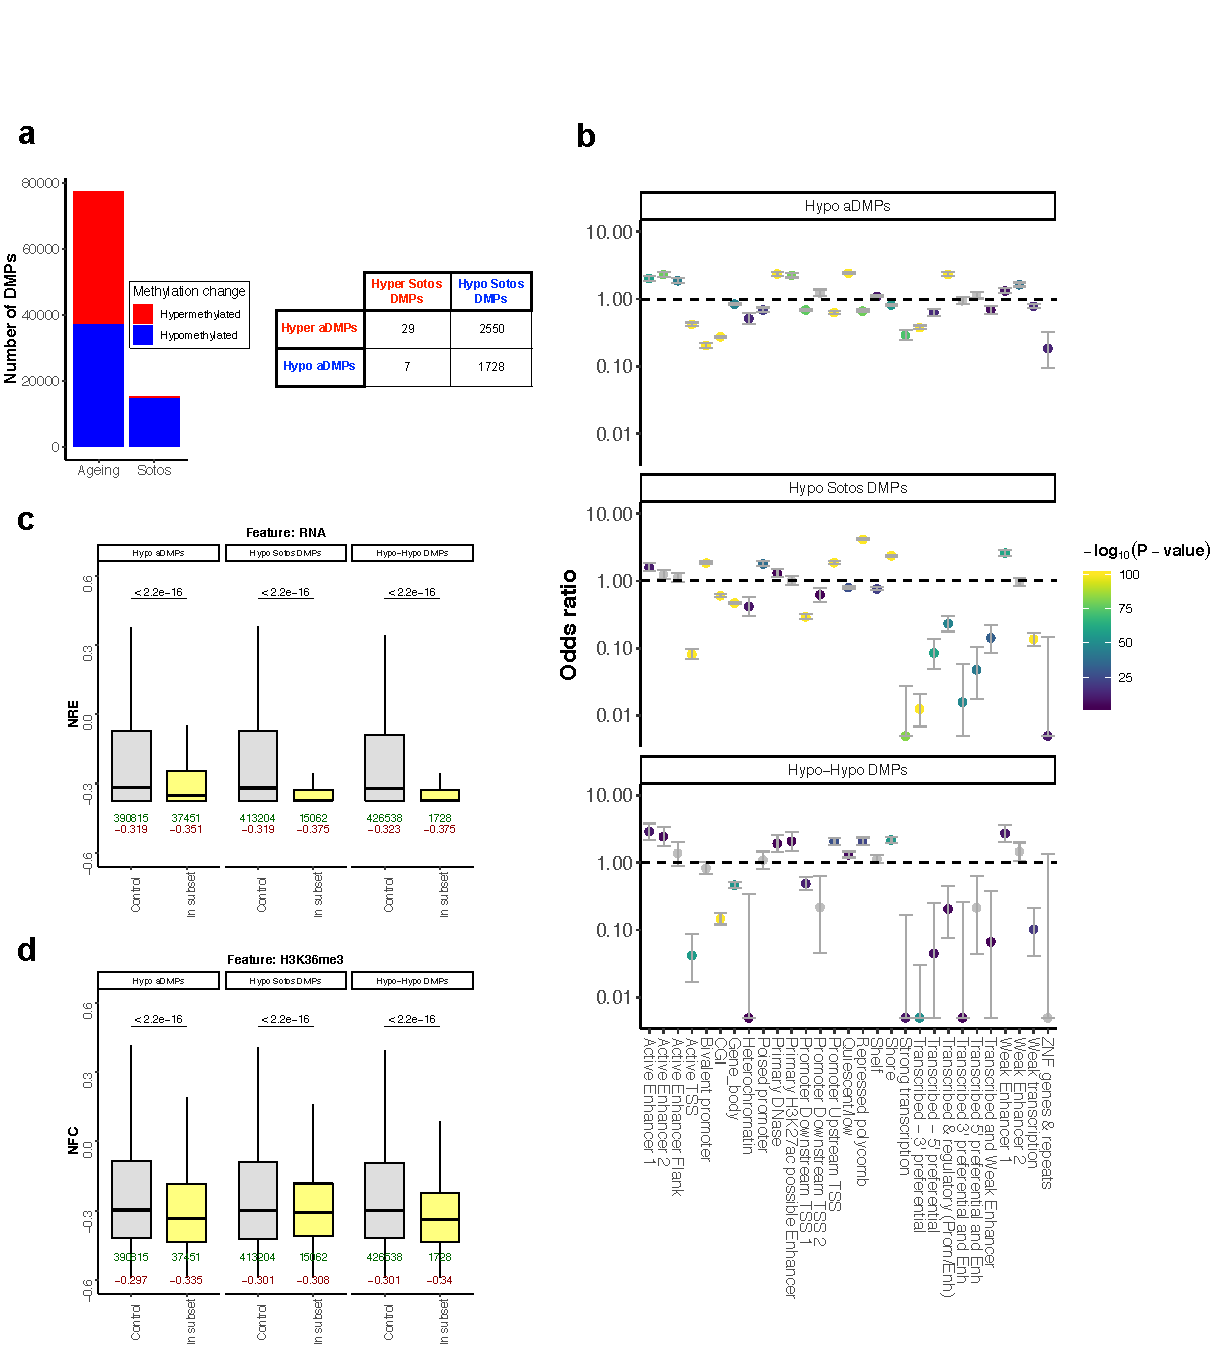
\includegraphics[width=1\textwidth]{C3_Fig5}
	\caption[Comparing DNA methylation changes in Sotos syndrome and physiological ageing]{Comparison between the DNA methylation changes during physiological ageing and in Sotos. \textbf{a.} On the left: barplot showing the total number of differentially methylated positions (DMPs) found during physiological ageing and in Sotos syndrome. CpG sites that increase their methylation levels with age in the healthy population or those that are elevated in Sotos patients (when compared with a control) are displayed in red. Conversely, those CpG sites that decrease their methylation levels are displayed in blue. On the right: table that represents the intersection between the ageing (aDMPs) and the Sotos DMPs. The subset resulting from the intersection between the hypomethylated DMPs in ageing and Sotos is called the `Hypo-Hypo DMPs’ subset (N=1728). \textbf{b.} Enrichment for the categorical (epi)genomic features considered when comparing the different genome-wide subsets of differentially methylated positions (DMPs) in ageing and Sotos against a control (see section~\ref{s:3.7}). The y-axis represents the odds ratio (\acrshort{OR}), the error bars show the 95\% confidence interval for the OR estimate and the colour of the points codes for $-\log_{10}(\text{p-value})$ obtained after testing for enrichment using Fisher's exact test. An OR > 1 shows that the given feature is enriched in the subset of DMPs considered, whilst an OR < 1 shows that it is found less than expected. In grey: features that did not reach significance using a significance level of $\alpha = 0.01$ after Bonferroni correction. \textbf{c.} Boxplots showing the distributions of the `normalised RNA expression' (\acrshort{NRE}) when comparing the different genome-wide subsets of differentially methylated positions (DMPs) in ageing and Sotos against a control (see section~\ref{s:3.7}). NRE represents normalised mean transcript abundance in a window of $\pm$ 200 bp from the CpG site coordinate (DMP) being considered. The p-values (two-sided Wilcoxon's test, before multiple testing correction) are shown above the boxplots. The number of DMPs belonging to each subset (in green) and the median value of the feature score (in dark red) are shown below the boxplots. \textbf{d.} As in c., but showing the `normalised fold change' (\acrshort{NFC}) for the H3K36me3 histone modification (representing normalised mean ChIP-seq fold change for H3K36me3 in a window of $\pm$ 200 bp from the DMP being considered).}
	\label{fig:c3_fig5}
\end{figure}


\bigskip

Then, I compared the intersections between the hypermethylated and hypomethylated DMPs in ageing and Sotos. Most of the DMPs were specific for ageing or Sotos (i.e. they did not overlap), but a subset of them were shared (table in Fig.~\ref{fig:c3_fig5}a). Interestingly, there were 1728 DMPs that became hypomethylated both during ageing and in Sotos (\textbf{`Hypo-Hypo DMPs'}). This subset of DMPs is of special interest because it could be used to understand in more depth some of the mechanisms that drive hypomethylation during physiological ageing. Thus, I tested whether the different subsets of DMPs are found in specific genomic contexts (Fig.~\ref{fig:sc3_fig4}, Fig.~\ref{fig:sc3_fig5}). DMPs that are hypomethylated during ageing and in Sotos were both enriched (odds ratio >1) in enhancer categories (such as `active enhancer 1' or `weak enhancer 1', see the chromatin state model used, from the K562 cell line, in section~\ref{s:3.7}) and depleted (odds ratio <1) for active transcription categories (such as `active TSS' or `strong transcription'), which was also observed in the `Hypo-Hypo DMPs' subset (Fig.~\ref{fig:c3_fig5}b). Interestingly, age-related hypomethylation in enhancers seems to be a characteristic of both humans \cite{Slieker2016,Slieker2018} and mice \cite{Cole2017}. Furthermore, both \textit{de novo} DNA methyltransferases (DNMT3A and DNMT3B) have been shown to bind in an H3K36me3-dependent manner to active enhancers \cite{Rinaldi2016}, consistent with these results.

\bigskip

When looking at the levels of total RNA expression (depleted for \acrshort{rRNA}) in blood, I confirmed a significant reduction in the RNA levels around these hypomethylated DMPs when compared with the controls sets (Fig.~\ref{fig:c3_fig5}c, see section~\ref{s:3.7} for more details on how the control sets were defined). Interestingly, hypomethylated DMPs in both ageing and Sotos were depleted from gene bodies (Fig.~\ref{fig:c3_fig5}b) and were located in areas with lower levels of H3K36me3 when compared with the control sets (Fig.~\ref{fig:c3_fig5}d, Fig.~\ref{fig:sc3_fig5}). Moreover, hypomethylated aDMPs and hypomethylated Sotos DMPs where both generally enriched or depleted for the same histone marks in blood (Fig.~\ref{fig:sc3_fig5}), which adds weight to the hypothesis that they share the same genomic context and could become hypomethylated through similar molecular mechanisms.

\bigskip

Intriguingly, I also identified a subset of DMPs (2550) that were hypermethylated during ageing and hypomethylated in Sotos (Fig.~\ref{fig:c3_fig5}a). These \textbf{`Hyper-Hypo DMPs'} seem to be enriched for categories such as `bivalent promoter' and `repressed polycomb' (Fig.~\ref{fig:sc3_fig4}), which are normally associated with developmental genes \cite{Bernstein2006,Bernhart2016}. These categories are also a defining characteristic of the hypermethylated aDMPs, highlighting that even though the direction of the DNA methylation changes is different in some ageing and Sotos DMPs, the genomic context in which they happen is shared.

\bigskip

Finally, I looked at the DNA methylation patterns in the 353 \textbf{Horvath's epigenetic clock CpG sites for the Sotos samples}. For each clock CpG site, I modelled the changes of DNA methylation with age in the healthy control individuals (0-55 years) and then calculated the deviations from these patterns for the Sotos samples (Fig.~\ref{fig:c3_fig6}, see equation~\ref{eq:3.4}). As expected, the landscape of clock CpG sites is dominated by hypomethylation in the Sotos samples, although only a small fraction of the clock CpG sites seems to be significantly affected (Fig.~\ref{fig:c3_fig6}c). Overall, I confirmed the trends reported for the genome-wide analysis (Fig.~\ref{fig:sc3_fig6}, Fig.~\ref{fig:sc3_fig7}, Fig.~\ref{fig:sc3_fig8}). However, given the much smaller number of CpG sites to consider in this analysis, very few comparisons reached significance.

\begin{figure}[htbp!] 
	\centering    
	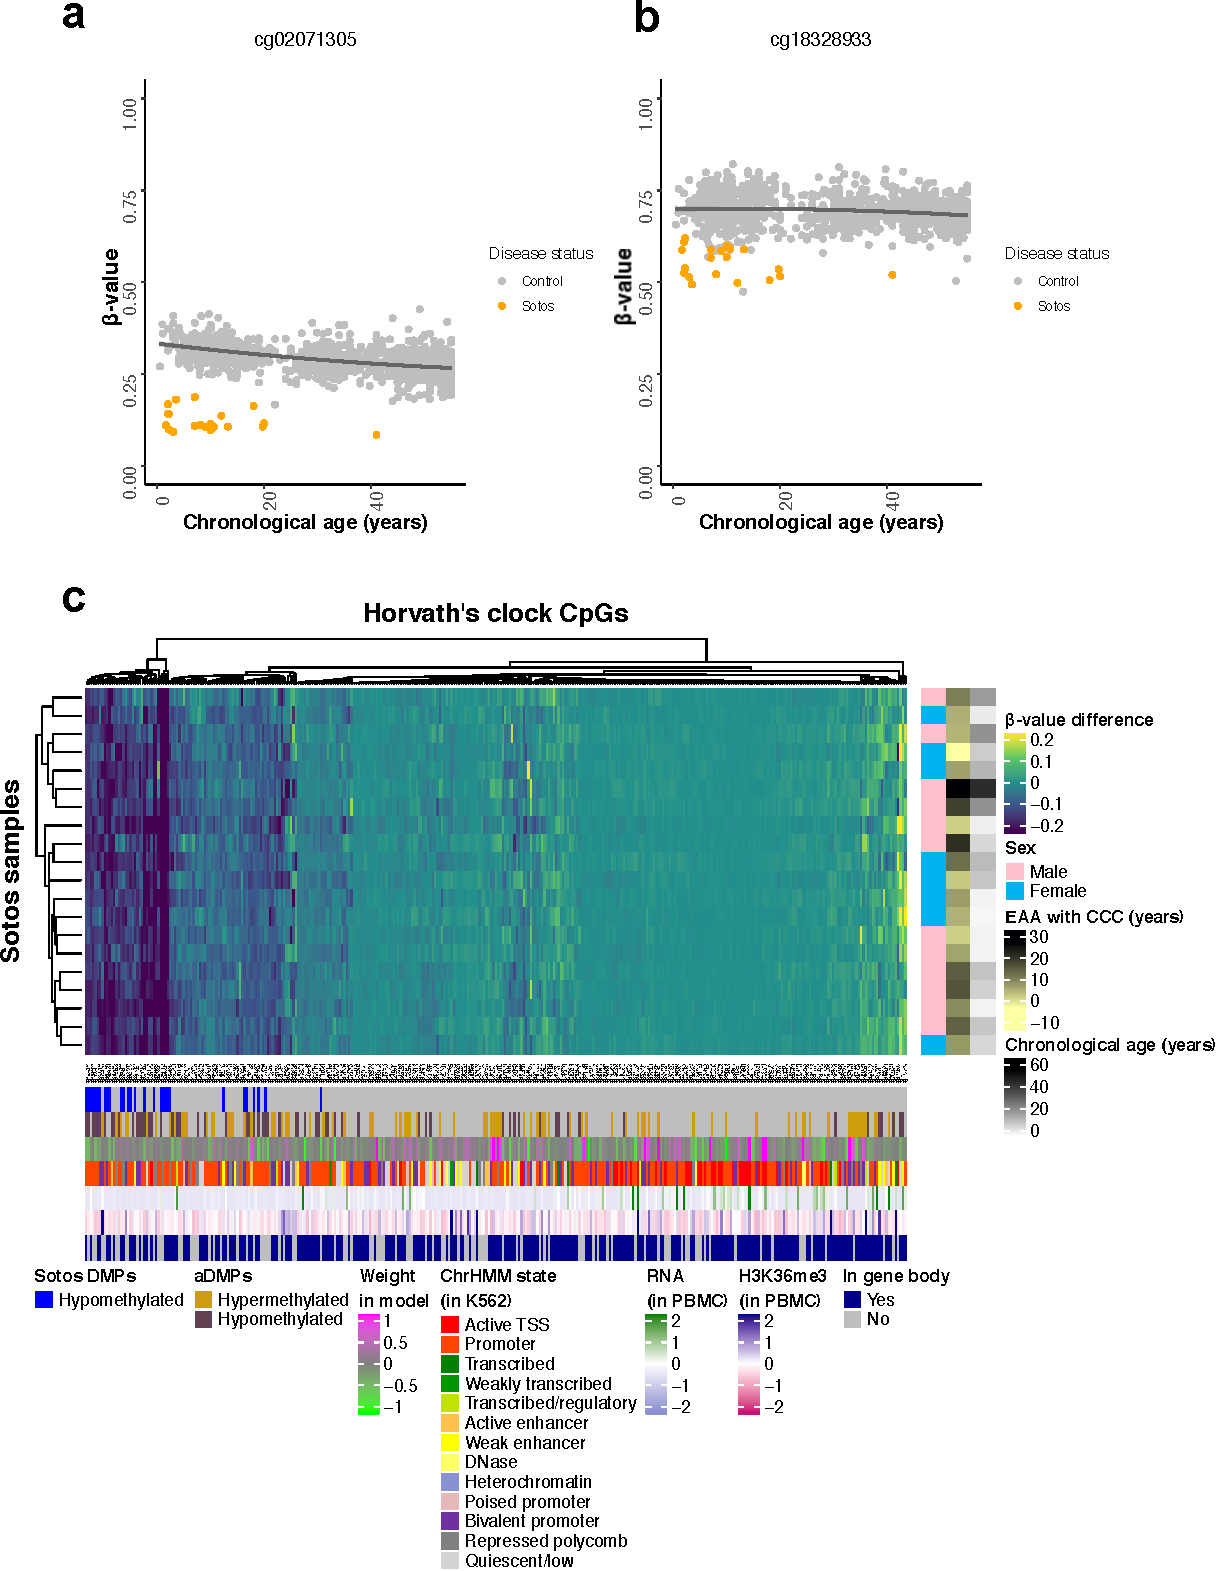
\includegraphics[width=1\textwidth]{C3_Fig6}
	\vspace*{1 mm}
	\caption[Landscape of Horvath's epigenetic clock CpGs in Sotos syndrome]{The landscape of Horvath's epigenetic clock CpG sites in Sotos syndrome. \textbf{a.} and \textbf{b.} DNA methylation ($\beta$-value) profiles for two of the clock CpG sites (cg02071305 and cg18328933). A linear model (displayed in dark grey, see equation~\ref{eq:3.4}) can be fixed to each CpG site to model the changes in $\beta$-value with chronological age in the controls (grey). Afterwards, the difference of the Sotos samples $\beta$-values (orange) with the controls can be estimated. \textbf{c.} Heatmap displaying the differential methylation patterns for Sotos samples (rows) when compared with controls in each one of the 353 epigenetic clock CpGs (columns). Hierarchical clustering was performed in both rows and columns. RNA refers to the `normalised RNA expression' (NRE). H3K36me3 refers to the H3K36me3 histone modification `normalised fold change' (NFC). aDMPs: differentially methylated positions during ageing. EAA: epigenetic age acceleration. CCC: cell composition correction. PBMC: peripheral blood mononuclear cells.}
	\label{fig:c3_fig6}
\end{figure}

\bigskip

I have demonstrated that the ageing process and Sotos syndrome share a subset of hypomethylated CpG sites that is characterised by an enrichment in enhancer features and a depletion of active transcription activity. This highlights the usefulness of \textbf{developmental disorders as a model to study the mechanisms that may drive the changes in the methylome with age}, since they permit stratification of the ageing DMPs into different functional categories that are associated with alterations in the function of specific genes and hence specific molecular components of the epigenetic ageing clock.

\smallskip

\section{Methylation Shannon entropy and the epigenetic clock}

\smallskip

In section~\ref{s:2.1.5} I have discussed how Shannon entropy can be applied in the context of DNA methylation data in order to measure the genome-wide epigenetic information loss that happens during ageing. It is possible to apply a methodology similar to the one described in section~\ref{s:2.2.2} to compare the methylation Shannon entropy in healthy controls (0-55 years) and Sotos patients (i.e. using a linear model similar to equation~\ref{eq:2.16}, although in this case the dependent variable is the entropy value). This allows testing whether Sotos syndrome patients present genome-wide Shannon entropy acceleration i.e. deviations from the expected genome-wide Shannon entropy for their age. Despite detailed analysis, I did not find evidence that this was the case when looking genome-wide (p-value = 0.71, Fig.~\ref{fig:c3_fig7}a,b, Fig.~\ref{fig:sc3_fig9}a).

\begin{figure}[htbp!] 
	\centering    
	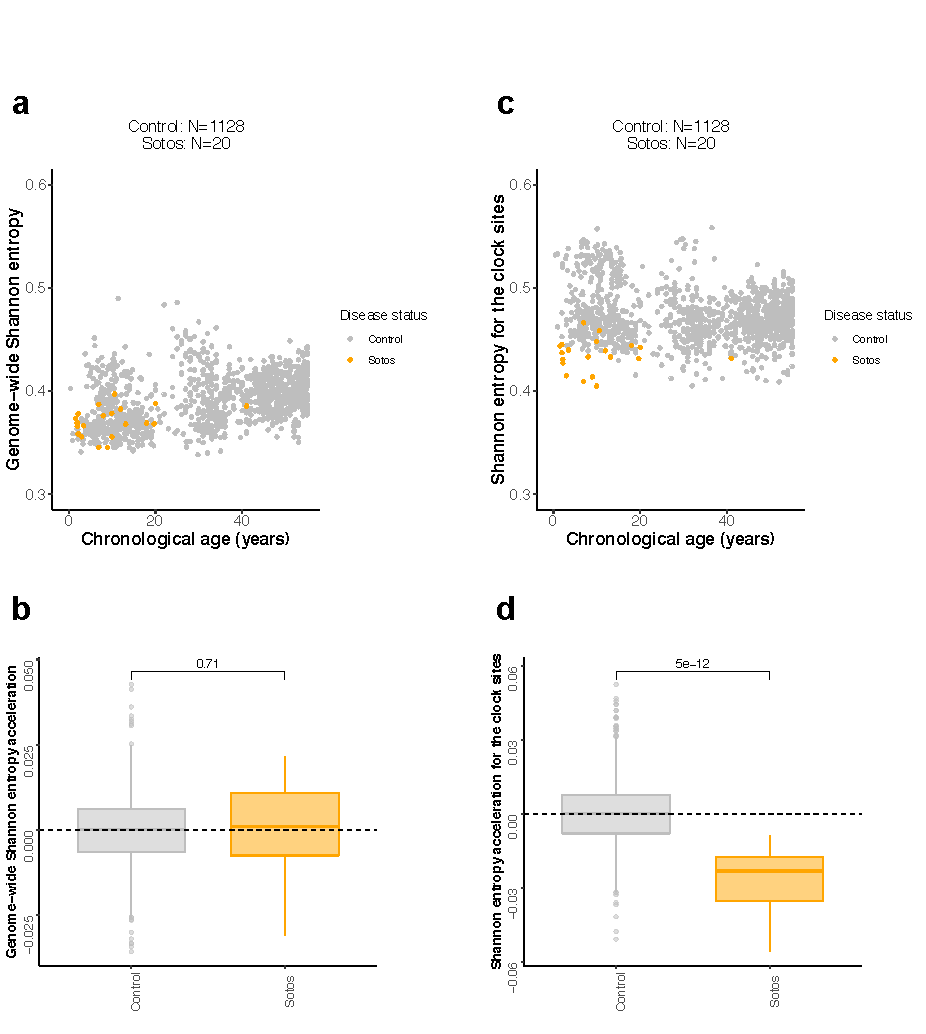
\includegraphics[width=1\textwidth]{C3_Fig7}
	\vspace*{1 mm}
	\caption[Methylation Shannon entropy during physiological ageing and in Sotos syndrome]{Analysis of methylation Shannon entropy during physiological ageing and in Sotos syndrome. \textbf{a.} Scatterplot showing the relation between genome-wide Shannon entropy (i.e. calculated using the methylation levels of all the CpG sites in the array) and chronological age of the samples for Sotos (orange) and healthy controls (grey). Each sample is represented by one point. \textbf{b.} Boxplots showing the distributions of genome-wide Shannon entropy acceleration (i.e. deviations from the expected genome-wide Shannon entropy for their age) for the control and Sotos samples. The p-value displayed on top of the boxplots was derived from a two-sided Wilcoxon’s test. \textbf{c.} As in a., but using the Shannon entropy calculated only for the 353 CpG sites in the Horvath's epigenetic clock. \textbf{d.} As in b., but using the Shannon entropy calculated only for the 353 CpG sites in the Horvath's epigenetic clock.}
	\label{fig:c3_fig7}
\end{figure}

\bigskip

When I considered only the 353 Horvath's epigenetic clock CpG sites for the entropy calculations, the picture was different. Shannon entropy for the 353 clock sites slightly decreased with age in the controls when I included all the batches, showing the opposite direction when compared with the genome-wide entropy (\acrshort{SCC} $= -0.1223$, p-value = 3.8166 $\cdot 10^{-5}$, Fig.~\ref{fig:c3_fig7}c). However, when I removed the `Europe' batch (which was an outlier even after pre-processing, Fig.~\ref{fig:sc3_fig10}), this trend was reversed and I observed a weak increase of clock Shannon entropy with age (\acrshort{SCC} $= 0.1048$, p-value = 8.6245 $\cdot 10^{-5}$). This shows that Shannon entropy calculations are very sensitive to batch effects, especially when considering a small number of CpG sites, and the results must be interpreted carefully, as already discussed in section~\ref{s:2.1.5}.

\bigskip

Interestingly, the mean Shannon entropy across all the control samples was higher in the epigenetic clock sites (mean = 0.4726, Fig.~\ref{fig:c3_fig7}c) with respect to the genome-wide entropy (mean = 0.3913, Fig.~\ref{fig:c3_fig7}a). Sotos syndrome patients displayed a lower clock Shannon entropy when compared with the control (p-value = 5.0449 $\cdot 10^{-12}$, Fig.~\ref{fig:c3_fig7}d, Fig.~\ref{fig:sc3_fig9}b), which is probably driven by the hypomethylation of the clock CpG sites. Furthermore, this highlights that the \textbf{Horvath's epigenetic clock sites could have slightly different characteristics in terms of the methylation entropy associated with them} when compared with the genome as a whole, something that to my knowledge has not been reported before.

\smallskip

\section{Discussion}

\smallskip

The epigenetic ageing clock has emerged as the most accurate biomarker of the ageing process and it seems to be a conserved property in mammalian genomes \cite{Horvath2018,Field2018}. However, it is still unknown whether the age-related DNA methylation changes measured are functional at all or whether they are related to some fundamental process of the biology of ageing. Developmental disorders in humans represent an interesting framework to look at the biological effects of mutations in genes that are fundamental for the integrity of the epigenetic landscape and other core processes, such as growth or neurodevelopment \cite{Aref-Eshghi2018,Bjornsson2015}. Therefore, using a reverse genetics approach, I aimed to identify genes that disrupt aspects of the behaviour of the epigenetic ageing clock in humans.

\bigskip

Most of the studies have looked at the epigenetic ageing clock using Horvath’s epigenetic clock \cite{Horvath2013}, and I decided to employ it as a tool to measure the epigenetic age of my samples. The results from the screen strongly suggest that Sotos syndrome accelerates epigenetic ageing. Sotos syndrome is caused by loss-of-function mutations in the NSD1 gene \cite{Choufani2015,Kurotaki2002}, which encodes a histone H3 lysine 36 (\acrshort{H3K36}) methyltransferase. This leads to a phenotype which can include pre-natal and post-natal overgrowth, facial gestalt, advanced bone age, developmental delay, higher cancer predisposition and, in some cases, heart defects \cite{Leventopoulos2009}. Remarkably, many of these characteristics could be interpreted as ageing-like, identifying \textbf{Sotos syndrome as a potential human model of accelerated physiological ageing}.

\bigskip

NSD1 catalyses the addition of either monomethyl (H3K36me) or dimethyl groups (H3K36me2) and indirectly regulates the levels of trimethylation (\acrshort{H3K36me3}) by altering the availability of the monomethyl and dimethyl substrates for the trimethylation enzymes (SETD2 in humans, whose mutations cause a `Sotos-like' overgrowth syndrome ) \cite{Wagner2012,Luscan2014}. H3K36 methylation has a complex role in the regulation of transcription \cite{Wagner2012} and has been shown to regulate nutrient stress response in yeast \cite{McDaniel2017}. Moreover, experiments in model organisms (yeast and worm) have demonstrated that \textbf{mutations in H3K36 methyltranferases decrease lifespan and, remarkably, mutations in H3K36 demethylases increase it} \cite{Ni2012,Sen2015,Pu2015}.

\bigskip

In humans, DNA methylation patterns are established and maintained by three conserved enzymes: the maintenance DNA methyltransferase DNMT1 and the \textit{de novo} DNA methyltransferases DNMT3A and DNMT3B \cite{Schubeler2015}. Both DNMT3A and DNMT3B contain PWWP domains that can read the H3K36me3 histone mark \cite{Dhayalan2010,Baubec2015}. Therefore, the H3K36 methylation landscape can influence DNA methylation levels in specific genomic regions through the recruitment of the \textit{de novo} DNA methyltransferases. Mutations in the PWWP domain of DNMT3A impair its binding to H3K36me2 and H3K36me3 and cause an undergrowth disorder in humans (microcephalic dwarfism) \cite{Heyn2019}. This redirects DNMT3A, which is normally targeted to H3K36me2 and H3K36me3 throughout the genome, to DNA methylation valleys (\acrshort{DMV}s, aka DNA methylation canyons), which become hypermethylated \cite{Heyn2019}; a phenomenon that also seems to happen during physiological ageing in humans \cite{Slieker2016,Rakyan2010,Teschendorff2010} and mice \cite{Cole2017}. DMVs are hypomethylated domains conserved across cell types and species, often associated with Polycomb-regulated developmental genes and marked by bivalent chromatin (with \acrshort{H3K27me3} and \acrshort{H3K4me3}) \cite{Xie2013,Long2013,Jeong2013,Li2018}. Therefore, I suggest a model (Fig.~\ref{fig:c3_fig8}) where the \textbf{reduction in the levels of H3K36me2 and/or H3K36me3, caused by a proposed decrease in H3K36 methylation maintenance during ageing or NSD1 function in Sotos syndrome, could lead to hypomethylation in many genomic regions (because DNMT3A is recruited less efficiently) and hypermethylation in DMVs (because of the higher availability of DNMT3A)}. Indeed, I observe enrichment for categories such as `bivalent promoter' or `repressed polycomb' in the hypermethylated DMPs in Sotos and ageing (Fig.~\ref{fig:sc3_fig4}), which is also supported by higher levels of Polycomb Repressing Complex 2 (\acrshort{PRC2}, represented by EZH2) and H3K27me3, the mark deposited by PRC2 (Fig.~\ref{fig:sc3_fig5}).This is also consistent with the results obtained for the epigenetic mitotic clock \cite{Yang2016}, where I observe a trend towards increased hypermethylation of Polycomb-bound regions in Sotos patients.

\begin{figure}[htbp!] 
	\centering    
	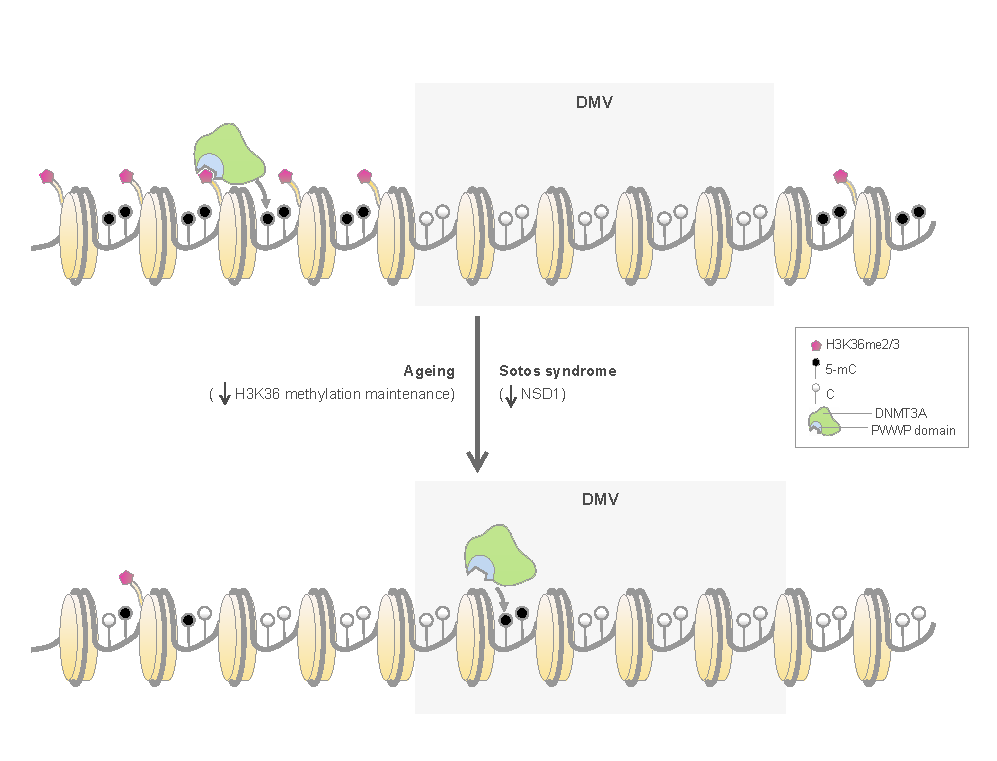
\includegraphics[width=1\textwidth]{C3_Fig8}
	\vspace*{1 mm}
	\caption[Proposed model that highlights the role of H3K36 methylation maintenance on epigenetic ageing]{Proposed model that highlights the role of H3K36 methylation maintenance on epigenetic ageing. The H3K36me2/3 mark allows recruiting \textit{de novo} DNA methyltransferases DNMT3A (in green) and DNMT3B (not shown) through their PWWP domain (in blue) to different genomic regions (such as gene bodies or pericentric heterochromatin) \cite{Baubec2015,Chantalat2011,Chen2004}, which leads to the methylation of the cytosines in the DNA of these regions (\acrshort{5mC}, black lollipops). On the contrary, DNA methylation valleys (\acrshort{DMV}s) are conserved genomic regions that are normally found hypomethylated and associated with Polycomb-regulated developmental genes \cite{Xie2013,Long2013,Jeong2013,Li2018}. During ageing, the H3K36 methylation machinery could become less efficient at maintaining the H3K36me2/3 landscape. This would lead to a relocation of \textit{de novo} DNA methyltransferases from their original \textit{genomic reservoirs} (which would become hypomethylated) to other non-specific regions such as DMVs (which would become hypermethylated and potentially lose their normal boundaries), with functional consequences for the tissues. This is also partially observed in patients with Sotos syndrome, where mutations in NSD1 potentially affect H3K36me2/3 patterns and accelerate the epigenetic ageing clock as measured with the Horvath's model \cite{Horvath2013}. Given that DNMT3B is enriched in the gene bodies of highly transcribed genes \cite{Baubec2015} and that I found these regions depleted in the differential methylation analysis, I hypothesise that the hypermethylation of DMVs could be mainly driven by DNMT3A instead. However, it is important to mention that my analysis does not discard a role of DNMT3B during epigenetic ageing.}
	\label{fig:c3_fig8}
\end{figure}

\bigskip

A recent preprint has shown that loss-of-function mutations in DNMT3A, which cause Tatton-Brown-Rahman overgrowth syndrome, also lead to a higher ticking rate of the epigenetic ageing clock \cite{Jeffries2018}. They also report positive epigenetic age acceleration in Sotos syndrome and negative acceleration in Kabuki syndrome, consistent with my results. Furthermore, they observe a DNA methylation signature in the DNMT3A mutants characterised by widespread hypomethylation, with a modest enrichment of DMPs in regions upstream of the transcription start site, shores and enhancers \cite{Jeffries2018}, which I also detect in the `Hypo-Hypo DMPs' (those that become hypomethylated both during physiological ageing and in Sotos). Therefore, \textbf{the hypomethylation observed in the `Hypo-Hypo DMPs' is consistent with a reduced methylation activity of DNMT3A}, which in my analysis could be a consequence of the decreased recruitment of DNMT3A to genomic regions that have lost H3K36 methylation (Fig.~\ref{fig:c3_fig8}).

\bigskip

Interestingly, H3K36me3 is required for the selective binding of the \textit{de novo} DNA methyltransferase DNMT3B to the bodies of highly transcribed genes \cite{Baubec2015}. Furthermore, DNMT3B loss reduces gene-body methylation, which leads to intragenic spurious transcription (aka cryptic transcription) \cite{Neri2017}. An increase in this so-called cryptic transcription seems to be a conserved feature of the ageing process \cite{Sen2015}. Therefore, the changes observed in the `Hypo-Hypo DMPs' could theoretically be a consequence of the loss of H3K36me3 and the concomitant inability of DNMT3B to be recruited to gene bodies. However, the `Hypo-Hypo DMPs' were depleted for H3K36me3, active transcription and gene bodies when compared with the rest of the probes in the array (Fig.~\ref{fig:c3_fig5}b-d), prompting me to suggest that the DNA methylation changes observed are likely mediated by DNMT3A instead (Fig.~\ref{fig:c3_fig8}). Nevertheless, it is worth mentioning that the different biological replicates for the blood H3K36me3 ChIP-seq datasets were quite heterogeneous and that the absolute difference in the case of the hypomethylated Sotos DMPs, although significant due to the big sample sizes, is quite small. Thus, I cannot exclude the existence of this mechanism during human ageing and an exhaustive study on the prevalence of cryptic transcription in humans and its relation to the ageing methylome should be carried out.

\bigskip

H3K36me3 has also been shown to guide deposition of the N$^6$-methyladenosine \acrshort{mRNA} modification (\acrshort{m$^6$A}), an important post-transcriptional mechanism of gene regulation \cite{Huang2019}. Interestingly, a decrease in overall \acrshort{m$^6$A} during human ageing has been previously reported in \acrshort{PBMC}s \cite{Min2018}, suggesting another biological route through which an alteration of the H3K36 methylation landscape could have functional consequences for the organism.

\bigskip

Because of the way that the Horvath epigenetic clock was trained \cite{Horvath2013}, it is likely that its constituent 353 CpG sites are a \textbf{low-dimensional representation of the different genome-wide processes that are eroding the epigenome with age}. My analysis has shown that these 353 CpG sites are characterised by a higher Shannon entropy when compared with the rest of the genome, which is dramatically decreased in the case of Sotos patients. This could be related to the fact that Horvath's clock CpGs are enriched in regions of bivalent chromatin (marked by H3K27me3 and H3K4me3), conferring a more dynamic or plastic regulatory state with levels of DNA methylation deviated from the collapsed states of 0 or 1. Interestingly, EZH2 (part of Polycomb Repressing Complex 2, responsible for H3K27 methylation) is an interacting partner of DNMT3A and NSD1, with mutations in NSD1 affecting the genome-wide levels of H3K27me3 \cite{Streubel2018}. Furthermore, Kabuki syndrome was weakly identified in my screen as having an epigenome younger than expected, which could be related to the fact that they show post-natal dwarfism \cite{Aref-Eshghi2017,Butcher2017}. Kabuki syndrome is caused by loss-of-function mutations in KMT2D \cite{Aref-Eshghi2017,Butcher2017}, a major mammalian H3K4 mono-methyltransferase \cite{Froimchuk2017}. Additionally, H3K27me3 and H3K4me3 levels can affect lifespan in model organisms \cite{Sen2016}. It will be interesting to test whether bivalent chromatin is a general feature of multi-tissue epigenetic ageing clocks.

\bigskip

Thus, \textbf{DNMT3A, NSD1 and the machinery in control of bivalent chromatin (such as EZH2 and KMT2D) contribute to an emerging picture on how the mammalian epigenome is regulated during ageing}, which could open new avenues for anti-ageing drug development. Mutations in these proteins lead to different developmental disorders with impaired growth defects \cite{Bjornsson2015}, with DNMT3A, NSD1 and potentially KMT2D also affecting epigenetic ageing. Interestingly, EZH2 mutations (which cause Weaver syndrome, Table~\ref{table:c3_table1}) do not seem to affect the epigenetic clock in my screen. However, this syndrome has the smallest number of samples ($N=7$) and this could limit the power to detect any changes.

\bigskip

My screen has also revealed that \textbf{Rett syndrome and fragile X syndrome (\acrshort{FXS}) could potentially have an accelerated epigenetic age}. It is worth noting that FXS is caused by an expansion of the CGG trinucleotide repeat located in the 5' \acrshort{UTR} of the FMR1 gene \cite{Schenkel2016}. Interestingly, Huntington's disease, caused by a trinucleotide repeat expansion of CAG, has also been shown to accelerate epigenetic ageing of human brain \cite{Horvath2016a}, pointing towards trinucleotide repeat instability as an interesting molecular mechanism to look at from an ageing perspective. It is important to notice that the conclusions for Rett syndrome, FXS and Kabuki syndrome were very dependent on the age range used in the healthy control (Fig.~\ref{fig:sc3_fig2}) and these results must therefore be treated with caution.

\bigskip

This study has several \textbf{limitations that I tried to address in the best possible way}. First of all, given that DNA methylation data for patients with developmental disorders is relatively rare, some of the sample sizes were quite small. It is thus possible that some of the other developmental disorders assessed are epigenetically accelerated but I lack the power to detect this. Furthermore, people with the disorders tend to get sampled when they are young i.e. before reproductive age. Horvath's clock adjusts for the different rates of change in the DNA methylation levels of the clock CpGs before and after adult/reproductive age (20 years in humans) \cite{Horvath2013}, but this could still have an effect on the predictions, especially if the control is not properly age-matched. My solution was to discard those developmental disorders with less than 5 samples and I required them to have at least 2 samples with an age $\geq$ 20 years, which reduced the list of final disorders included to the ones listed in Table~\ref{table:c3_table1}. 

\bigskip

Future studies should increase the sample size and follow the patients during their entire lifespan in order to confirm these findings. Furthermore, it would be interesting to identify mutations that affect, besides the mean, the variance of epigenetic age acceleration, since changes in methylation variability at single CpG sites with age have been associated with fundamental ageing mechanisms \cite{Slieker2016}. Finally, testing the influence of H3K36 methylation on the epigenetic clock and lifespan in mice will provide deeper mechanistic insights.

\smallskip

\section{Additional methods} \label{s:3.7}

\subsection*{Sample generation and annotation}

I collected DNA methylation data generated with the Illumina Infinium HumanMethylation450 BeadChip (450K array) from human blood. In the case of the developmental disorder samples, I combined public data with data generated in-house by my collaborators in Canada (Table~\ref{table:s2_table1}, Fig.~\ref{fig:sc3_fig1}). The wet-lab protocols used in the public datasets can be found in their respective GEO repositories. DNA methylation data from my Canadian collaborators was generated according to the manufacturer's protocol \cite{Research,Illumina2015}.

\bigskip

Basic metadata (including the chronological age) was also stored. All the mutations in the developmental disorder samples were manually curated using Variant Effect Predictor \cite{McLaren2016} in the GRCh37 (\acrshort{hg19}) human genome assembly. Those samples with a variant of unknown significance that had the characteristic DNA methylation signature of the disease were also included (they are labelled as `YES\_predicted' in Fig.~\ref{fig:sc3_fig1}). In the case of fragile X syndrome (\acrshort{FXS}), only male samples with full mutation (>200 repeats) \cite{Schenkel2016} were included in the final screen. As a consequence, only samples with a clear molecular and clinical diagnosis were kept for the final screen.

\subsection*{Identifying differentially methylated positions in Sotos syndrome} 

Following a strategy similar to the one outlined in section~\ref{s:2.1.4}, I identified those array probes that were differentially methylated in patients with Sotos syndrome. I compared the Sotos samples (N=20) against the internal control samples (N=51) from the same dataset (GSE74432) \cite{Choufani2015}, fitting the following linear model to each one of the array probes:

\begin{align} \label{eq:3.1}
Beta \sim Disease\_status + Age + Sex+ Gran + CD4T + CD8T + B + Mono + NK + PC1 + ... + PC17
\end{align} 

where $Beta$ is the $\beta$-value for the array probe being evaluated; $Disease\_status$ indicates whether a sample comes from a healthy individual (0) or a Sotos syndrome patient (1); $Age$ is the chronological age (in years) of the samples; $Sex$ encodes for the sex of the samples (0/1); $Gran$, $CD4T$, $CD8T$, $B$, $Mono$ and $NK$ are the cell type proportions from the samples as calculated with my cell-type deconvolution strategy and $PCN$ is the $N$th principal component that captures technical variance and accounts for potential batch effects (see section~\ref{s:2.2.3} for more details).

\bigskip

P-values and regression coefficients were extracted for the $Disease\_status$ covariate. I selected as my final Sotos DMPs those CpG probes that survived the analysis after Bonferroni multiple testing correction with a significance level of $\alpha=0.01$. 

\subsection*{(Epi)genomic annotation of the CpG sites}

Different (epi)genomic features were extracted for the CpG sites of interest. All the data were mapped to the \textit{hg19} assembly of the human genome.
The \textbf{continuous features} were calculated by extracting the mean value in a window of $\pm$ 200 bp from the CpG site coordinate using the \textit{pyBigWig} package \cite{Richter}. I chose this window value based on the methylation correlation observed between neighbouring CpG sites in previous studies \cite{Zhang2015}. The continuous features included (Fig.~\ref{fig:sc3_fig11}):

\begin{itemize}
	
	\item ChIP-seq data from ENCODE (histone modifications from peripheral blood mononuclear cells or \acrshort{PBMC}; EZH2, as a marker of Polycomb Repressing Complex 2 binding, from B cells; RNF2, as a marker of Polycomb Repressing Complex 1 binding, from the K562 cell line). I obtained Z-scores (using the \textit{scale} function in R) for the values of `fold change over control' as calculated in ENCODE \cite{Consortium2012}. When needed, biological replicates of the same feature were aggregated by taking the mean of the Z-scores in order to obtain the `normalised fold change' (\acrshort{NFC}).
	
	\item ChIP-seq data for LaminB1 (GSM1289416, quantified as `normalised read counts' or \acrshort{NRC}) and \acrshort{Repli-seq} data for replication timing (GSM923447, quantified as `wavelet-transformed signals' or \acrshort{WTS}). I used the same data from the IMR90 cell line as in \cite{Zhou2018}.
	
	\item Total RNA-seq data (\acrshort{rRNA} depleted, from PBMC) from ENCODE. I calculated Z-scores after aggregating the `signal of unique reads' (\textit{\acrshort{sur}}) for both strands (+ and - ) in the following manner:
	
	\begin{align}
	RNA_i = \log_2(1 + sur_{i+} + sur_{i-})
	\end{align}
	
	where $RNA_i$ represents the RNA signal (that then needs to be scaled to obtain the `normalised RNA expression' or \acrshort{NRE}) for the $i$th CpG site.
	
\end{itemize}

The \textbf{categorical features} were obtained by looking at the overlap (using the \textit{pybedtools} package) \cite{Quinlan2011} of the CpG sites with the following:

\begin{itemize}
	
	\item Gene bodies, from protein-coding genes as defined in the basic gene annotation of GENCODE release 29 \cite{Frankish2018}.
	
	\item CpG islands (\acrshort{CGI}s) were obtained from the UCSC Genome Browser \cite{Bock2007}. Shores were defined as regions 0 to 2 kb away from CGIs in both directions and shelves as regions 2 to 4 kb away from CGIs in both directions as previously described \cite{Zhang2015,Martin-Herranz2017a}.
	
	\item Chromatin states were obtained from the K562 cell line in the Roadmap Epigenomics Project (based on imputed data, 25 states, 12 marks) \cite{Consortium}. A visualisation for the association between chromatin marks and chromatin states can be found in \cite{Consortiuma}. When needed for visualisation purposes, the 25 states were manually collapsed to a lower number of them.
	
\end{itemize}

I compared the different genomic features for each one of the subsets of CpG sites (hypomethylated aDMPs, hypomethylated Sotos DMPs, ...) against a control set. This control set was composed of all the probes from the background set from which I removed the subset that I was testing. In the case of the comparisons against the 353 Horvath clock CpG sites, a background set of the 21368 (21K) CpG probes used to train the original Horvath model \cite{Horvath2013} was used. In the case of the genome-wide comparisons for ageing and Sotos syndrome, a background set containing all 428266 probes that passed my pre-processing pipeline was used (see section~\ref{s:2.1.2}).

\bigskip

For each continuous feature, the feature score distributions for a given subset of CpG sites and the control set were compared using the non-parametric two-sided Wilcoxon's test. For each categorical feature, I first created a $2x2$ contingency table, with the two variables indicating whether a given CpG site overlaps with the categorical feature under consideration (Yes/No) and whether the CpG site is in the subset (e.g. hypomethylated aDMPs) being considered (Yes/No). Using Fisher's exact test (as implemented in the \textit{fisher.test} function in R) I calculated the p-value and the odds ratio (\acrshort{OR}), which allows determining whether the categorical feature under consideration is enriched in the CpGs subset. 

\subsection*{Differences in the epigenetic clock CpGs $\beta$-values for Sotos syndrome}

To compare the $\beta$-values of the Horvath clock CpG sites between the healthy samples and Sotos samples I fitted the following linear model to each array probe from the Horvath's epigenetic clock (353 in total) in the healthy individuals samples (Fig.~\ref{fig:c3_fig6}a,b):

\begin{align} \label{eq:3.4}
Beta \sim Age+Age^2+Sex+Gran+CD4T+CD8T+B+Mono+NK+PC1+... +PC17
\end{align}

where $Beta$ is the $\beta$-value for the clock array probe being evaluated; $Age$ is the chronological age (in years) of the samples; $Sex$ encodes for the sex of the samples (0/1); $Gran$, $CD4T$, $CD8T$, $B$, $Mono$ and $NK$ are the cell type proportions from the samples as calculated with my cell-type deconvolution strategy and $PCN$ is the $N$th principal component that captures technical variance and accounts for potential batch effects (see section~\ref{s:2.2.3} for more details). The $Age^2$ covariate allows accounting for non-linear relationships between chronological age and the $\beta$-values.

\bigskip

Finally, I calculated the difference between the $\beta$-values in Sotos samples and the predictions from the models in equation~\ref{eq:3.4} and displayed these differences in an annotated heatmap (Fig.~\ref{fig:c3_fig6}c).   

